% Define document class
\documentclass[twocolumn]{aastex631}
\usepackage{showyourwork}

% \usepackage[dvipsnames]{xcolor}
% \usepackage[colorlinks]{hyperref}
% \usepackage{colortbl}
\usepackage{multirow}
\definecolor{pyBlue}{RGB}{31, 119, 180}
\definecolor{pyRed}{RGB}{214, 39, 40}
\definecolor{pyGreen}{RGB}{44, 160, 44}

% Link setup
% \newcommand\myshade{80}
% \hypersetup{
%   linkcolor  = pyGreen!\myshade!black,
%   citecolor  = pyBlue!\myshade!black,
%   urlcolor   = pyRed!\myshade!black,
%   colorlinks = true
% }

\newcommand{\jax}{\texttt{JAX}\xspace}
\newcommand{\ripple}{\texttt{ripple}\xspace}
\newcommand{\lalsuite}{\texttt{lalsuite}\xspace}
\newcommand{\CC}{C\nolinebreak\hspace{-.05em}\raisebox{.4ex}{\tiny\bf +}\nolinebreak\hspace{-.10em}\raisebox{.4ex}{\tiny\bf +}}

\newcommand{\TE}[1]{{\color{pyGreen} #1}}
\newcommand{\te}[1]{\textbf{\color{pyGreen}(TE: #1)}}
\definecolor{rb4}{HTML}{27408B}
\newcommand{\kw}[1]{{\color{rb4}[KW: #1 ]}}

% Begin!
\begin{document}

% Title
\title{\ripple: Differentiable Waveforms for Gravitational Wave Data Analysis}

\newcommand{\JHU}{\affiliation{William H. Miller III Department of Physics and Astronomy, Johns Hopkins University, Baltimore, Maryland 21218, USA}} 
\newcommand{\OKC}{\affiliation{The Oskar Klein Centre, Department of Physics, Stockholm University, AlbaNova, SE-106 91 Stockholm, Sweden}} 
\newcommand{\NORDITA}{\affiliation{Nordic Institute for Theoretical Physics (NORDITA), 106 91 Stockholm, Sweden}}
\newcommand{\UdeM}{\affiliation{Département de Physique, Université de Montréal, 1375 Avenue Thérèse-Lavoie-Roux, Montréal, QC H2V 0B3, Canada}} 
\newcommand{\Mila}{\affiliation{Mila -- Quebec AI Institute, 6666 St-Urbain, \#200, Montreal, QC, H2S 3H1}} 
\newcommand{\CGP}{\affiliation{Center for Gravitational Physics, University of Texas at Austin, Austin, TX 78712, USA}}
\newcommand{\CCA}{\affiliation{Center for Computational Astrophysics, Flatiron Institute, New York, NY 10010, USA}}

% Author list
\author{Adam Coogan} \UdeM \Mila
\author{Thomas D.~P.~Edwards} \JHU \OKC \NORDITA
\author{Daniel Foreman-Mackey} \CCA
\author{Maximiliano Isi} \CCA
\author{Kelvin Lam} \CCA
\author{Kaze W.~K.~Wong} \CCA
\author{Aaron Zimmerman} \CGP

% Abstract with filler text
\begin{abstract}
    Since their discovery in 2015, gravitaitonal waves (GWs) have developed into a unique observational probe used throughout fundamental and astro-phyics.
    As more detections continue, data analysis taks are becoming increasingly computationally demanding.
    Here we propose the use of automatic differentiation through the programming framework \jax for accelerating a variety of these analsyis tasks.
    Firstly, we demonstrate that highly accurate waveforms (IMRPhenomD) can be written in \jax and demonstrate that the evaluation speed of the waveform (and its derivative) is not substantially slower than the \lalsuite implenetation in \CC.
    We then focus on three applications where speed and differentiable waveforms are essential.
    Firstly, we demonstrate that stochastic gradient descent can be used to optimize the $\sim 200$ coefficients that make up the waveform. 
    In particular, we demonstrate that the typical \textit{match} with numerical relativiely waveforms can be improved by more than 30\% without any additional overhead.
    Secondly, we show that Fisher forecasting calculations can be sped up by $\sim 100\times$ with no loss in accuracy.
    This increased speed makes population forecasting substantially simpler, as discussed extensively in \citep{Iacovelli:2022bbs, Iacovelli:2022mbg}.
    Finally, we show that gradient based samplers like Hamiltonian Monte Carlo can improve acceptance rates of XXX. 
    Since differentiable waveforms appear to have substatial advantages for a variety of tasks throughtout GW science (with little downside), we propose that waveform developers use \jax to build new waveforms moving forward.
    Our waveform code, called \ripple, can be found at XXX, and will continue to be updated with new waveforms as they are formulated.

\end{abstract}

\section{Introduction}
\label{sec:intro}

% Intro outline
% - What are gravitational waves and what are data analysis tasks?
% - What are derivatives, and how can they be used?
% - What is automatic differentiation, and why has it become particularly useful now? JAX?
% - Discussion of what waveforms are most ameanable to being differentiable
% - In this paper

The discovery of gravitational waves (GWs) from inspiraling and mergering compact objects (COs) has revolutionized our understanding of both fundamental physics and astronomy~\citep{LIGOScientific:2021djp}.
Although the data volumes from GW detectors are relatively small, analyzing the data is a computationally demanding task.
In addition, this computational cost will substatially increase when next generation detectors come online.
The complexity begins before data gathering where one is required to generate banks of template waveforms which will be used for a matched-filter search~\citep{Owen:1998dk, Owen:1995tm}. 
Once potential candidates are found, parameter estimation (PE) is performed to extract the detailed source properties of each event.
In the most minimial example, this requires a Markov Chain Monte Carlo (MCMC) on an 11 dimensional parameter space for each event.
Beyond this simple scenario, more complex waveform models with many additional parameters may be used to test for deviations from General Relativity.
Finally, using the results of the PE, population synthesis models constrain the progenitors systems from which the black holes we see merging today began their journey~\citep{Wong:2022flg}.
All of these tasks require significant compute.
In this paper, we will argue that differentiable waveforms (and more generally differentiable pipelines) can play a significant role in alleaviating this computational demand.

Derivatives are ubiqitously useful throughout data analysis tasks.
For instance, during PE, derivative information can be used to guide the sampling towards regions with higher likelihood values (e.g. in Hamiltonian Monte Carlo~\citep{2017arXiv170102434B} or Gradient Decsent).
Gradients are particularly valuable for high dimensional spaces.
Unfortunately, in the field of GW data analysis, analytic derivatives of the necessary quantities (such as the likelihood) have historically been difficult to obtain.
Numerical derivatives also suffer from accuracy issues stemming from rounding or truncation errors.
However, recent progress in automatic differentiation (AD) has shown promise in allowing general, fast derivative calcuations for gravitational waveforms~\citep{Coogan:2022qxs}.

Automatic differentiaton is a family of methods used to compute machine precision derivatives with little computational ovearhead. 
AD's recent ascendance is primarily driven by its use in machine learning, particularly for derivative computations of neural networks which use gradient descent during training.
The core idea of AD is that any mathematical function can be broken down into a small set of basic operations, each with a known differentiation rule.\footnote{
    Of course, non-differentiable functions exist and care must be taken when treating these special cases.
    }
The full derivative can then be contructed using the chain rule.
There are now a variety of AD implementations, most notably in deep learning frameworks such as \texttt{pytorch}~\citep{pytorch} and \texttt{tensorflow}~\citep{tensorflow2015-whitepaper}.
More general frameworks exist in \texttt{julia}~\citep{zygote, forwarddiff}, although \texttt{julia}'s limited support in GW physics precludes its general use.
Here we make use of \jax~\citep{jax2018github} due to its easy integration with \texttt{python} libraries and its just-in-time (JIT) compiler which allows the same code to run on a variety of hardware accelerators (i.e. GPUs).

There are a variety of gravitational waveforms currently used in analysis pipelines.
They are generally structured into different families, the most common of which are: the effective-one-body (EOB), the phenomenological inspiral-merger-ringerdown (IMRPhenom), and numerical relativity surrogate (NRsurrogate).
Of these, the IMRPhenom family is most well suited for an AD implementation in \jax.
In particular, its closed form expression and fixed size frequency grid make a \jax implementation that complies with the constraints of JIT compilation simple.
EOB waveforms on the other hand require... \te{Max or Kaze, could one of you write something about why its hard? I don't know enough about EOB.}

In this paper we argue that differentiable waveforms will be a vital component for the future of GW data analysis.
In addition, we present \ripple, a small GW \texttt{python} package which can serve as a respository for differentiable implementations of some of the main waveforms currently used in LIGO and Virgo analyses. 
The remainder of this paper is structured as follows. 
In Sec.~\ref{sec:waveforms} we discuss the differentiable waveforms implemented in \ripple and perform some benchmarks to demonstrate the speed and accruacy of the derivative calculations. 
In Sec.~\ref{sec:applications} we discuss three distinct applications using differentiable waveforms. 
Firstly, we illustrate how the fit coefficients that form part of the IMRPhenom waveform models could be improved by high dimensional fitting, enabled by a differentiable waveform. 
Secondly, we implement differnetiable detector response functions and show that the speed of Fisher matrix calculations can be substantially improved using AD.
Finally, we run an illustrative injection example using Hamiltonian Monte Carlo to demonstrate that the acceptance rate of derivative samplers is substantially larger than traditional MCMCs.
The associated code can be found at \ripple~\citep{ripple}.

\section{Differentiable Waveforms}
\label{sec:waveforms}

A variety of waveform families have been developed to accurately model the GW emission from COs. 
When the COs are relatively well separated, the dynamics of the system can be well approximated with post-Newtonian expansion.
However, close to merger, numerical relatively simulations are required to accurately model the binary.
Unfortunately, these numerical simulations are computationally expensive and cannot be run in conjunction with data analysis.
Approximate, phenomenological waveforms have therefore been constructued to enable relatively fast waveform generation at sufficient accuracy.

As mentioned in the previous section, the three major waveform families that have been developed to date are:  EOB,  NRsurrogate, and IMRPhenom.
Note that unlike NRsurrogate, both the EOB and PhenomIMR waveforms are calibrated to numerical relativity waveforms.
EOB waveforms require one to model the binary system using a Hamiltonian and are typically slow to evaluate whereas IMRPhenom waveforms are constructed with simple closed-form expressions.
IMRPhenom waveforms are therefore ideally suited for AD, espeically using \jax. 
In this paper we focus mainly on the aligned spin circular orbit model IMRPhenomD~\citep{Husa:2015iqa, Khan:2015jqa}.

The implementation of IMRPhenomD in \lalsuite is in C, and therefore needs to be rewritten natively into \texttt{pyhton} to be compatible with \jax.
We have re-written IMRPhenomD from scratch using a combination of pure \texttt{pyhton} and \jax derivatives.
In addition, we have restructed the code for readability and evaluation speed as well as exposing the internal fitting coefficients to the user (which we will use later in Sec.~\ref{sec:applications}).

To demonstrate our implempation of IMRPhenomD is faithful to the \lalsuite implementation, we start by defining the noise weighted inner product:
\begin{equation}
    \left(h_{\theta_1}|h_{\theta_2}\right) \equiv 4 \, \mathrm{Re} \int^{\infty}_{0} \mathrm{d} f \, \frac{ h_{\theta_1}(f) h^*_{\theta_2}(f)}{S_n(f)}\, ,
\end{equation}
where $S_n$ is the (one-sided) noise power spectral density (PSD) and $h_{\theta_1}$ is the frequency domain waveform evaluated at the instrinsic parameter point $\theta_1$.
We can then normalize the inner product through
\begin{equation}
    \left[h_{\theta_1}|h_{\theta_2}\right] = \frac{\left(h_{\theta_1}|h_{\theta_2}\right)}{\sqrt{\left(h_{\theta_1}|h_{\theta_1}\right)\left(h_{\theta_2}|h_{\theta_2}\right)}}\, .
\end{equation}
Now we are ready to define the \textit{match} which is given by 
\begin{equation}
    \mathrm{m}(h_{\theta_1}|h_{\theta_2}) \equiv \max_{t_c,\, \phi_c} \left[h_{\theta_1} \, \middle| \, h_{\theta_2} \right]\,
\end{equation}
where $t_c$ and $\phi_c$ are, respectively, the time and phase of coalesence.

Since the match is a measure of the difference between two waveforms, we can use it to demonstrate that the implementation of IMRPhenomD in \ripple accurately matches the \lalsuite implementation.
This is shown in Fig.~\ref{fig:match}, where we have calculated the $\mathrm{m}(h_{\theta_1}|\bar{h}_{\theta_1})$ across the entire parameter space.\footnote{
    Specifically, we use 2000 points in the ranges $m_{1,2} = (1,50)\,M_{\odot}$ and $\chi_{1,2} = (-1,1)$. In addition, we evaulated the waveforms on a frequency grid from $32\,$Hz to $1024\,$Hz with frequency spacing $\Delta f = 0.0125 \,$Hz.
}
Here, $h_{\theta_1}$ corresponds to the \ripple waveform implementation and $\bar{h}_{\theta_1}$ is the \lalsuite implementation. 
From Fig.~\ref{fig:match}, it is clear that the \ripple waveform matches with the \lalsuite waveform to numerical precision across the majority of the parameter space.
In particular, the blue points indicate parameter points where the $1-\mathrm{m}(h_{\theta_1}|h^{*}_{\theta_1})=0$ and would therefore not appear in the log scale colorbar.
\begin{figure}[t]
    \script{random_matches.py}
    \begin{centering}
        \includegraphics[width=\linewidth]{figures/random_matches.pdf}
        \caption{
            Match between the \ripple and \lalsuite implementations of the IMRPhenomD waveform as a function of total mass and effective spin.
            \te{Need to investigate more?}
        }
        \label{fig:match}
    \end{centering}
\end{figure}

There remains some slight deviation between the two waveform implementations at low total mass. \te{Do I need to look more into this...? The discussion below looks odd with this plot}
This is likely due to the fact that cubic interpolators, which are used within IMRPhenomD to calculate the ringdown and damping frequencies, are not currently supported in \jax.
Instead, we initially use \texttt{scipy}'s cubic interpolator to create a fine grid of XXX values, which we then linearly interpolate during waveform generation.
Unfortunately, we cannot make the initial cubic interpolation arbitrarily fine as this would add additional computational overhead when loading the data during waveform evaluation.
The remaining error in the waveform at high masses is therefore primarily down to the coarseness in this interpolation.
Note however, that the differences are well below the accuracy requirements of the waveforms and will have no noticeable for realistic data analysis tasks.

For maximum utility, a waveform needs to be fast to evaluate.
Fortunately, the IMRPhenom waveforms are constructed from simple closed-form expressions which are computationally efficient.
Since the \lalsuite implementation of IMRPhenomD is written in \texttt{C}, the evaluation of the waveform itself is faster than \ripple.
Benchmarking on a MacBook Pro with an M1 Max Apple Silicon processor, we find that a single waveform evaluation takes $\sim 2-5\,\mathrm{ms}$ for \lalsuite (interfaced with python) and $\sim 5-8\,\mathrm{ms}$ for \ripple.\footnote{
    For this benchmark we used $16\,\mathrm{Hz}$ and $1024\,\mathrm{Hz}$ for the lowest and highest frequencies respectively. 
    In addition, we used a frequency spacing of $0.0125\,\mathrm{Hz}$. 
    We performed this benchmark by evaluating the waveform $5000$ times and taking the average evaluation time.
}
Although slower on a CPU benchmark, a key advantage of using \jax is its native ability to run on a GPU.
Waveform calls can therefore be evaluated in parallel, massively improving performance.
Performing the same benchmark as above on a google colab notebook with the freely provided GPU, we find that on average waveform evaluations take $\sim 0.00005\mathrm{ms}$, nearly five orders of magnitude faster.
Generalizing \lalsuite waveforms to run on a GPU would be a significant undertaking.

The primary arguement of this paper is that waveform derivatives will also be highly vauable to data analysis tasks. 
AD provides two big advantages when it comes to evaluating derivatives compared to numerical differentiation.
First, the accuracy of derivatives from AD are signficantly more stable than finite difference methods.
In particular, finite differences suffer from both rounding and truncation errors, meaning that the user is required to \textit{tune} the width over which the difference is taken.
On the other hand, AD produces machine precision derivatives with no tuninig.
Second, AD scales favourably with the dimensionality of the function.
In particular, for every input dimension, $D$, added one would need to evaluate the function at least $2D$ times to calcuate finite difference derivatives for all input parameters.
For reverse mode AD, one only needs two function calls to evaluate the derivative of all input parameters, regardless of dimenison.\footnote{
    Note that although the number of function calls is small, reverse mode AD does add memory overhead.
    We've not found this to be limiting in any of the situations tested so far.
}
Since the parameter space of GWs in General Relativity (GR) has $\mathcal{O}(10)$ dimensons, the speed of derivative evaluation is less crucial than the stability.
However, this might change for waveforms in beyond GR models where many more parameters are added.

Overall, we have demonstrated that the IMRPhenom waveform family is ideally suited for AD.
Moreover, we have shown that our implementation of IMRPhenomD in \ripple is accurate and quick to evaluate, especially when hardware acceleration is available.
In the next section, we will discuss a variety of potential use cases of differentiable waveforms.

% Emphasise the stability of gradients. $Done$
% Not just a faster way of evaluating PhenomD. $Done$
% Change plot to be q vs chieff. $Done$
% Note that lalsuite cannot be made massively parallel on GPUs. $Done$
% Don't need a full section on Fisher, but make sure to mention. People love Fisher.
% Use acceptance rate as a good explanation of speed ups
% Wall time a messy comparison. Based too much off of hardware
% Emphasise that gradients are beneficial

\section{Applications}
\label{sec:applications}

Here, we will illustrate how three core tasks in GW science can be substantially improved through the use of differentiable waveforms.
In the paper we will primarily look at toy examples, leaving a more careful analyses to future work. 
The three tasks discussed here cover a wide range of GW science, starting with waveform development all the way to forecasting and parameter estimation.

\subsection{Finetuning Waveform Coefficients}
\label{subsec:coeffs}

% \te{Kelvin should add stuff here}

Having an accurate waveform model is essential for many data analysis tasks in
GW, such as searching for signals and estimating source parameters given data.
While waveforms generated using numerical relativity simulations are commonly
regarded as the most accurate, they are too computationally expensive to be used
in any practical data analysis tasks. To create waveform models that can be used
in data analysis, there are a number of groups creating "approximants" of the
full numerical relativity waveforms, which are essentially simpler ansatzes that
are not as accurate but can be evaluated much faster. There are a few families
of approximants, such as the IMRPhenom family, SEOB family, and the NRSurrogate
model. \kw{cite and add a couple more sentences to introduce the waveform
families.} \te{I think a full dicussion of the various waveform families just belongs in section 2, so don't need too much more here I'd say.}

Every waveform approximant has some fitting coefficients that are fixed during
the process of calibrating the ansatz to NR waveforms. In the case of
IMRPhenomD, there are 209 fitting coefficients used to capture the separate
behavior of the amplitude and phase as a function of the mass ratio and spins.
The accuracy of fitting coefficients determines how well the approximant
reproduces the NR waveform. The inaccuracy in obtaining the fitting coefficients
means misrepresentation of the NR waveform, meaning the use of approximant will
introduce some systematic error in downstream data analysis task. For example, sufficiently large systematic errors 
would mean cause the recovered source parameters to be biased in the case of PE.

% Motivation
Previously in the construction of IMRPhenomD \citep{Khan:2015jqa}, waveform
coefficients are fitted in segments with amplitude and phase separated.
Individual segments are then connected together such that they are
differentiable. Using this method, the generated waveforms are expected to be
erroneous, as the connections would affect the originally fitted segments. The
coefficients of the current IMRPhenomD implementation are often hand tuned, and
are tuned in sub-sets of parameters instead of all together. This means the
tuning process ignore the correlation between different sub-sets of parameters,
so the best-fitted solution obtained by fitting sub-sets of parameters may not
be the global optimum compared to fitting all coefficients at once. Instead, by
jointly fitting all coefficients, the inaccuracy in fitting individual and
connecting different segments can be accounted during the optimization.
Therefore, there is potential accuracy one can gain by fitting all coefficients
at once.

\kw{Kelvin Fill}
Since we can differentiate through the entire waveform model against the fitting
parameters, one can use gradient descent to find the optimal fitting parameters
all at once instead of fitting them in subsets.

Here, we define the mismatch as
\begin{equation}
	\mathcal{M}=1-\mathrm{m}(h_{\mathrm{IMR}}|h_{\mathrm{NR}}), 
\end{equation} 
In our optimization procedure, we took NR waveforms stated in \citep{Khan:2015jqa} as training waveforms to fit waveform coefficients. 
By defining the mean of individual mismatches as the loss function for optimization, we can calibrate the set of coefficients using gradient descent. 

\kw{Describe figure losscompare}

\begin{figure}[t]
\centering
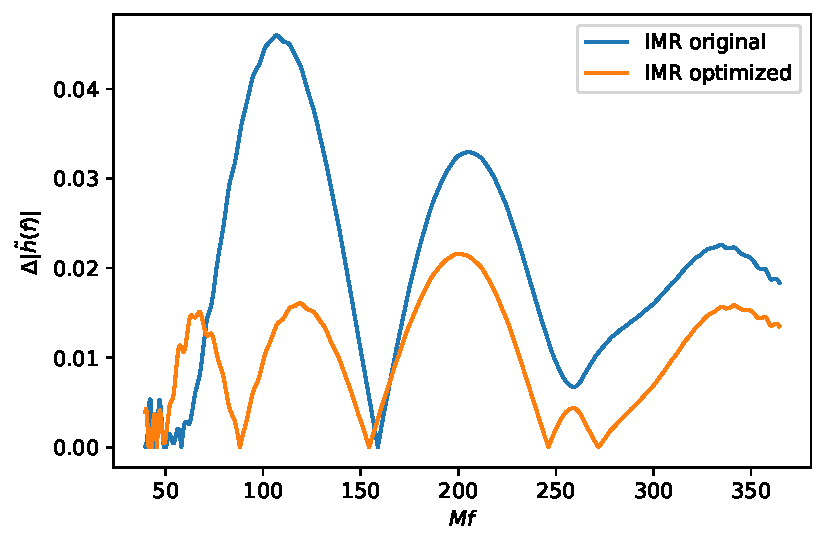
\includegraphics[width=\linewidth]{../static/amplitude_loss.pdf}
\caption{Relative error of amplitudes of IMRPhenomD waveforms. Blue: Error
    between original Phenom waveform and NR waveform; Orange: Error between
    optimized waveform and NR waveform. \te{Can you add the data and the plotting script to the repo so that we can generate the plots using the same matplotlib settings?}}
\label{fig:loss_compare}
\end{figure}

\kw{Describe figure logdiff}
As demonstration, Fig. \ref{fig:loss_compare} shows the relative error of original and optimized waveform at different frequencies. 
In general, the error of optimized waveform is lower than that of the original waveform. 
The error in the early inspiral region is substantially decreased by half and other regions also show good improvement in accuracy.   

\begin{figure}[t]
\centering
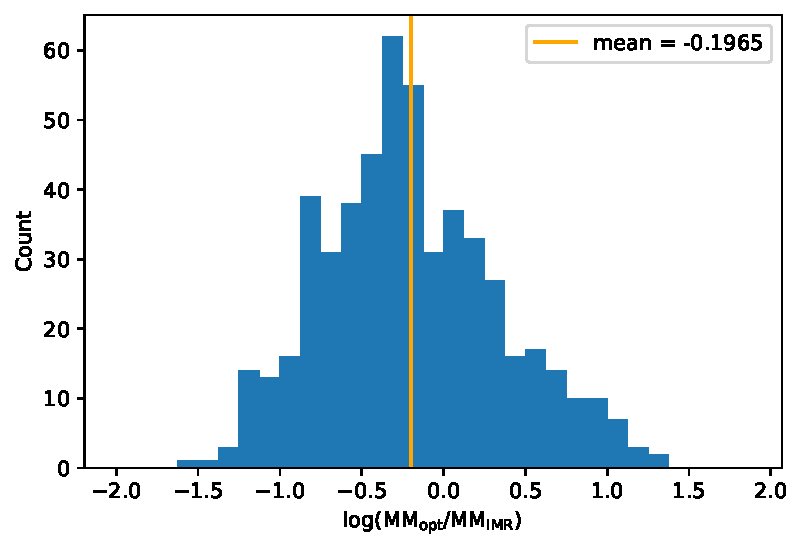
\includegraphics[width=\linewidth]{../static/MM_logdiff_q148_LIGO.pdf}
\caption{Distribution of the log difference of mismatches between optimized
    and original model. The mean shows a 36\% decrease in mismatch. }
\label{fig:MM_logdiff}
\end{figure}


Instead of examining individual waveforms, we investigate the general behavior of mismatches for a set of testing waveforms. 
In Fig. \ref{fig:logdiff_q148}, the distribution of log difference of mismatches are shown. 
The distribution mean lies towards the negative side, which indicates a improvement in the model. 
Despite there are testing waveforms that performed worse after optimization, it is verified that the ansatz of IMRPhenomD does not fit well with most of these waveforms, hence cannot be improved by optimization.  
Therefore, the new set of waveform coefficients can produce better waveforms for GW analyses. 

\kw{Describe implication}
% Implication

This fine-tuning step is rather simple and general. Given a different
differentiable waveform model, one can apply the same procedure to optimize the
coefficients in the new model, i.e. applying gradient descent to optimize all
the fitting coefficients all together. This provides a more flexible control
during the calibration process, and potentially better final result.
With further modifications to the optimization process, the set of waveform
coefficients can be retuned to give almost an order-of-magnitude improvement.
\kw{Where is the proof for this?} 


\subsection{Fisher Forecasting}
\label{subsec:fisher}

\begin{figure}[t!]
    \script{sky_localization.py}
    \centering
    \includegraphics[width=\linewidth]{figures/sky_localization.pdf}
    \caption{
        This plot should show a sky localization error bar.
    }
    \label{fig:sky_localization}
\end{figure}

Forecasting the sensitivity of future experiments is an essential task in GW science.
Due to its theoretical simplicity and evaluation speed, the Fisher matrix formalism is commonly deployed to estimate how well a binary system's parameters can be measured.
The Fisher matrix approach is built around the assumption of a Gaussian likelihood.
Although in practice this assumption is often violated in real GW datasets, the results obtained using a Fisher analysis can provide quick and useful diagnotistics in evaluating sensitivities for a variety of models and detector configurations.

Computing the Fisher matrix requires one to evaluate derivatives of the likelihhood which in turn involves derivatives of the waveform model and detector projection functions.
AD is therefore perfectly suited for computing Fisher matrices accurately and efficiently. 
Forecasting with Fisher matrices for third generation detectors has already been extensively explored in \citep{Iacovelli:2022bbs, Iacovelli:2022mbg}.
Here we purely want to illustrate the simplicitly and speed of AD for forecasting rather than providing new physics insights.
We therefore consider a simple, three detector setup corresponding to the two LIGO detectors in addition to Virgo.

The Fisher information matrix for a single detector is typically given by 
\begin{equation}
    \mathcal{I}^{k}_{ij} = (\partial_i h_0 | \partial_j h_0) \, ,
\end{equation}
where $k$ indicates the detector, $\partial_i = \partial/\partial \theta_i$, and $h_0$ is the strain measured by the detector which is given by,
\begin{equation}
    h_0(\theta) = F_+(\lambda) h_{+}(\phi) + F_\times(\lambda) h_{\times}(\phi) \, .
\end{equation}
Note that here we have separated out the intrinsic ($\phi$) and extrinsic ($\lambda$) variables as well as introducing the detector projection functions for the plus and cross polarizations as $F_+$ and $F_\times$ respectively.
Since we are considering a three detector setup we simply add the Fisher matrices from the individual detectors to get the combined Fisher matrix:
\begin{equation}
    \mathcal{I}_{ij} =  \mathcal{I}^{\mathrm{Hanford}}_{ij} + \mathcal{I}^{\mathrm{Livingston}}_{ij} + \mathcal{I}^{\mathrm{Virgo}}_{ij}   \, .
\end{equation}
Finally, we invert the Fisher matrix to calculate the covariance matrix.

% \begin{table*}[ht!]
%     \begin{center}
%     \begin{tabular}{c|c|c|c|c|c|c|c|c}
%     \hline\hline
%     \hfil $\boldsymbol{m_1, m_2}$ &
%     \hfil $\boldsymbol{\chi_1, \chi_2}$ &
%     \hfil $\boldsymbol{D}$ &
%     \hfil $\boldsymbol{t_c}$ &
%     \hfil $\boldsymbol{\phi_c}$ &
%     \hfil $\boldsymbol{\iota}$ &
%     \hfil $\boldsymbol{\psi}$ &
%     \hfil $\boldsymbol{RA}$ &
%     \hfil $\boldsymbol{DEC}$
%     \\
%     \hline\hline
%     \hfil [0.1, 3] &
%     \hfil [0, 1] &
%     \hfil [0, 1] &
%     \hfil [0.7, 1.3] &
%     \hfil [-3, 0] &
%     \hfil [0, 3] &
%     \hfil [-3, 3] &
%     \hfil [-3, 3] &
%     \hfil [-3, 3]
%     \\
%     \hline\hline
%     \end{tabular}
%     \end{center}
%     \caption{caption here}
%     \label{tab:priors}
% \end{table*}

\begin{table}[t]
    % \begin{center}
    \centering
    \begin{tabular}{c|c}
    \hline\hline
    $m_1, m_2$ & $\boldsymbol{U}[1.0, 50]\, \mathrm{M}_\odot$ \\ \hline
    $\chi_1, \chi_2$ & [-0.99, 0.99] \\ \hline
    $D$ & [500, 1000]\, Mpc \\ \hline
    $t_c$ & 0.0 \\ \hline
    $\phi_c$ & 0.0 \\ \hline
    Inclincation Angle, $\iota$ & $\boldsymbol{U}[0, 1]$ \\ \hline
    Polarization Angle, $\psi$ & $\boldsymbol{U}[0, 1]$ \\ \hline
    Right Ascension, $\delta$ & $\boldsymbol{U}[0, 1]$ \\ \hline
    Declination, $\alpha$ & $\boldsymbol{U}[0, 1]$ \\ 
    \hline\hline
    \end{tabular}
    % \end{center}
    \caption{Priors for the 11 dimensional parameter space used for the Fisher forecasting population analysis in Sec.~\ref{subsec:fisher}. 
    $\boldsymbol{U}$ indicates a uniform distribution between the two variables in the brackets.}
    \label{tab:priors}
\end{table}

To illustrate the computational speed of computing Fisher matrices with AD, we consider a population of binaries and compute the sky localtization error following Eq.~(28) in \citep{Iacovelli:2022bbs, Iacovelli:2022mbg}.
Since the Fisher matrix approach is known to have both theoretical issues as well as numerical instabilities for low signal-to-noise events, we restrict our population to only nearby systems.
A full list of the distributions used to generate the various parameters in our population are given in Tab.~\ref{tab:priors}.
The resulting population produces binaries with signal-to-noise ratios ranging from $\mathcal{O}(10-10^2)$.

The distribution of sky localization errors from a population of $10^3$ binaries can be seen in Fig.~\ref{fig:sky_localization}.
We have verified that our errors agree with a separate dedicated Fisher forecasting code~\citep{Borhanian:2020ypi} to within X percent.
This demonstrates that AD can be used to accurately produce population level forecasts.

Moreover, each error calculation (including computing the Fisher matrices for each detector and the inversion procress) is substantially faster.
In particular, we find that after compilation each error calculation takes approximately half a second on a single computing core.
\texttt{GWbench}~\citep{Borhanian:2020ypi}, on the other hand, takes $\mathcal{O}$(minutes) for each Fisher calculation using the same detector setup and frequency grid.
This factor of over 100 speed up is substantial considering the fact that a single core evaluation of the \ripple waveform is significantly slower that the \lalsuite call.
As discussed above, performance can be further improved by utilising hardware acceleration such as parallel GPU processing.
AD therefore represents a fast and accurate way of performing population level analyses, and should be utilized for testing the capabilities of next generation detectors.

\subsection{Derivative Based Samplers - Hamiltonian Monte Carlo}
\label{subsec:hmc}

After the search algorithms have constructed a list of confidently detected binaries, the next step is to sample from the posterior of each sources parameters - so called parameter estimation (PE).
To do this, one typically uses a Markov Chain Monte Carlo (MCMC) sampler or nested sampler~\citep{multinest, dynesty}.
Although robust, both MCMC and nested sampling are slow to converge and are known to perform poorly in high dimensional parameter spaces.
For example, sampling the 15 dimensional parameter space for a BBH system can take $\mathcal{O}(10)$hours, whilst BNS systems can take up to weeks.
Dedicated fast samplers have been designed to get approximate posteriors on the sky localization to faciliate follow-up electromagnetic observations.
Nevertheless, these do not present the whole picture; fast, general parameter estimation therefore remains a primary goal of GW data analysis.

A primary issue with both MCMC and nested sampling is that neither utlizes information about the likelihood's derivative and must therefore randomly walk towards areas of highest likelihood.
Derivative based samplers, on the other hand, have been shown to extrapolate well to higher dimensions although they sometimes come with their own drawbacks.
Here we simply aim to demonstrate the utility of a derivative based sampler and their efficiency on a small test problem.
In particular, we will show that proposals made using an Hamiltonian Monte Carlo (MC) sampler are accepted at a much higher rate than a traditional MCMC algorithm.
In a follow up paper we will demonstrate that minute scale PE can be achieved by exploiting normalizing flows~\citep{2022arXiv221106397W, Gabrie:2021tlu} together with a derivative based sampler~\citep{PEpaper}.


\section{Discussion and Conclusion}
\label{subsec:discussion}

In this paper we introduced and discussed the various benefits of differentiable waveforms in \jax for GW data analysis.
First, we demonstrated the speed and accuracy of our implementation of the aligned spin IMRPhenomD waveform.
In particular, we showed that it matches the \lalsuite implementation to near machine precision and can be easily parallelized on a GPU, making waveform calls up to five orders of magnitude faster.
Second, we discussed three data analysis tasks which can all be substantially improved by utlizing derivative information of the waveform.
Although we primarily discuss toy examples in this paper, each can be extended to the full data analysis task, some of which will be shown in upcoming papers~\citep{PEpaper}.
Differentiable waveforms therefore represent a crucial tool to perform efficient GW science.

Currently the biggest constraint to adopting differentiable waveforms is the need to re-write the most commonly used waveforms into \jax (or pure python).
In order to showcase the benefits of differentiable waveforms as quickly as possible, at the time of writing, we have only implemented an aligned spin GW model (IMRPhenomD).
We plan on adding a variety of different waveforms to \ripple in the near future with the primary goal of reaching a \jax version of a fully precessing, higher order mode waveform such as IMRPhenomXPHM.
Ideally, future waveforms should be implemented either in pure python or using \jax directly.
This would ensure that the community can easily utilize differentiability and hardware acceleration in the future.

In this paper, we have primarily focussed on the IMRPhenom family of waveforms as their closed form expression is perfectly suited for implementation in \jax.
Two other waveform families are commonly used in GW data analysis: the effective-one-body (EOB) and numerical relativity surrogate (NRSurrogate). 
Some progress has been made towards the construction of a differentiable NRsurrogate, currently it seems difficult to implement EOB waveforms in \jax.
In particular, the evolution of the Hamiltonian required to evaluate an EOB waveform is both inherently slow to differentiate and difficult to implement in \jax which requires fixed length arrays for its JIT compilation.
Since EOB waveforms are often regarded as the state-of-the-art, more work is required to see if a fast, differentiable implementation is possible.

\te{End on a final good thing?}

\section{Acknowledgments}
This work was supported by collaborative visits funded by the Cosmology and Astroparticle Student and Postdoc Exchange Network (CASPEN). 
T.E. is supported by the Horizon Postdoctoral Fellowship.

\bibliography{bib}

\end{document}
